\documentclass[main.tex]{subfiles}
\begin{document}
\section{LSTM-RNN}
This section will try to provide the necessary theory behind recurrent neural networks, focusing on the \textit{Long Short Term Memory} model (LSTM). Such recurrent models are the generally the default methods which are chosen to work on sequential data such as in time series prediction. This explanation should hopefully give an idea as to how these types of models are used for predicting time series and why they are suitable for the problem in this project. Lastly, the results of the models performance on the power consumption data set are presented, showing the capabilities of the LSTM. 

\subsection{Theory}
A recurrent neural network (RNN) is a model for processing sequences of data, and contrary to simpler feed forward neural networks where a sequence of data would be processed and have weights and features learned separately, a recurrent neural network can share weights across a sequence. Hereby lies the strength of an RNN as this parameter sharing can lead to generalization across sequences. An important feature of this type of model is that each member of the output is a result of the previous output, thereby giving the model its name \cite{Goodfellow-et-al-2016}. Below, figure \ref{fig:RNN unfolded} shows on the left a circuit diagram of the input entering state \textit{$h$} and the recurrence with a time delay of a single step shown by the clock. On the right the circular diagram is unfolded showing each state at time step \textit{$t$} as being a result of the previous state at \textit{$t-1$} as well as the input at step \textit{$t$}.

\begin{figure}[H]
\centering
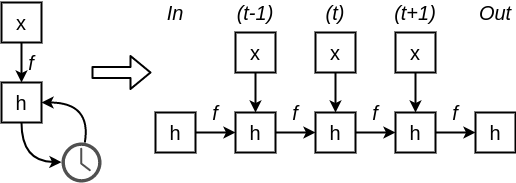
\includegraphics[width=0.8\textwidth]{Figures/rnnunfold.png}
\caption{Unfolded recurrent network with no output}
\label{fig:RNN unfolded}
\end{figure}

Like most neural networks, in between the input and the output layer lies the hidden layers. These consist of cells holding the weights that are given to the inputs and fed through the network. After each hidden layer, a function is applied which alters or shapes the output given to the next layer, this is an activation function. These building blocks can then be put together to form the neural network.
\\
\textit{Backpropagation} is used to calculate the gradient with respects to the loss function and the model parameters of a network. In the case of a recurrent network, the specific algorithm that is used is called \textit{backpropagation through time}, as the model parameters are shared throughout the network and the output at a single timestep depends on the previous timesteps, and the gradients need to be calculated recursively \cite{Goodfellow-et-al-2016}.\\
However, this recurrent nature can lead to a problem, which is very general when working with deeper neural networks, which is where one could start to observe vanishing or exploding gradients \cite{Goodfellow-et-al-2016}. A vanishing or exploding gradient occurs when training the model using backpropagation, the model weights are updated by multiplying with a value corresponding to the partial derivative of the loss functions with respects to the weights in the current iteration. Now, for deep architectures, this means that very small or very big weights could potentially be multiplied with themselves many times, thus leading to weight values that either become so small or so big that they vanish or explode\cite{Goodfellow-et-al-2016}.\\
\\
One approach to solving this problem is using a form of RNN called a \textit{gated network}, and more specifically the LSTM model.\\
The core of the LSTM lies in the introduction self-loops and gates confined within a LSTM cell, which helps to control the information flow \cite{Goodfellow-et-al-2016}. The self-loop is an internal recurrence within a cell and there is still the overall recurrent nature of the network. 

\begin{figure}[H]
\centering
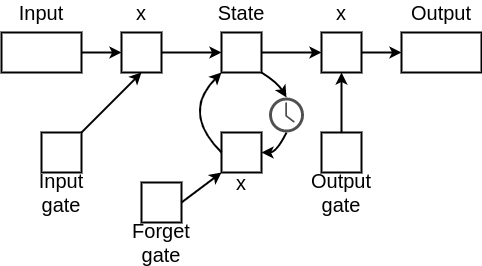
\includegraphics[width=0.6\textwidth]{Figures/LSTMCell.png}
\caption{LSTM Cell}
\label{fig:LSTM Cell}
\end{figure}

The external input gate, $g_i^{(t)}$, controls whether the value of the input itself is computed into the state through a \textit{Sigmoid} activation function. 
$$g_i^{(t)} = \sigma (b_i^g + \sum_j U_{i,j}x_j^{(t)} + \sum_j W_{i,j}h_j^{(t-1)})$$
Within the self-loop is the state unit which is controlled by the forget gate, $f_i^{(t)}$, also using a \textit{Sigmoid} activation function, and it looks as follows:
$$f_i^{(t)} = \sigma (b_i^f + \sum_j U^f_{i,j}x_j^{(t)} + \sum_j W^f_{i,j}h_j^{(t-1)})$$
here \textit{$x$} is the current input vector and \textit{$h$} is the current hidden layer vector. $b^f$, $U^f$, and $W^f$ are the biases, input weights, and recurrent weights for the forget gate respectively.\\
The state cell, $s_i^{(t)}$, is then computed, with the conditional self-loop, as:
$$s_i^{(t)} = f_i^{(t)}s_i^{(t-1)} + g_i^{(t)} \sigma (b_i^f + \sum_j U^f_{i,j}x_j^{(t)} + \sum_j W^f_{i,j}h_j^{(t-1)})$$
where \textit{$b$}, \textit{$U$}, and \textit{$W$} are the biases, input weights, and recurrent weights from the input cell.\\
All the while, the output gate, $q_i^{(t)}$, can shut off the cells output completely, and is also using a \textit{Sigmoid} activation function.
$$q_i^{(t)} =  \sigma (b_i^o + \sum_j U^o_{i,j}x_j^{(t)} + \sum_j W^o_{i,j}h_j^{(t-1)})$$
again $b^o$, $U^o$, and $W^o$, being the biases, input weights, and recurrent weights for the output gate.
Together, these functions make up for the output, $h_i^{(t)}$, of the whole LSTM cell:
$$h_i^{(t)} = \text{tanh}(s_i^{(t)})q_i^{(t)}$$
In theory, this should make a recurrent neural network, in the form of a LSTM, suitable for time series forecasting. However, despite the fact that this type of model should be able to learn longer dependencies, it might struggle on predicting many steps ahead while keeping a high amount of precision.

\subsection{Implementation}
The LSTM model was implemented using \texttt{pytorch}, and in the simplest form of this type of model, with a single LSTM layer. For the other hyperparameters, which are the learning rate and the number of hidden layers, a grid search was run, finding the best combination of learning rates of $\{0.1,0.01,0.001\}$ and number of hidden layers $\{10,50,100,200\}$. Generally, the best learning rate seemed to be 0.01, and the number of hidden layers fluctuated between 50 and 200.
\\
For training the model, and evaluating it, the data was split into 60\%/20\%/20\% training, validation, and testing respectively. And also done in batches of around 36.\\
In training the model, a form of adaptive stopping was run, which trained the model until no improvement in validation loss was seen for a patience amount of 40 epochs. This was set relatively high, hoping that the model would possibly improve over a longer period of time, also with the knowledge that this type of model usually runs a decent amount of epochs, however as will be seen below it did not make much of a difference.

\subsection{LSTM Results}
Below in this section, the results from different runs of the LSTM model can be seen, with different examples of multi-step predictions, showing the capabilities of the LSTM model. The first predictions are made with 50 days and predicting 25 days ahead, and the next ones are predicting 50 days ahead.

\begin{figure}[H]
\centering
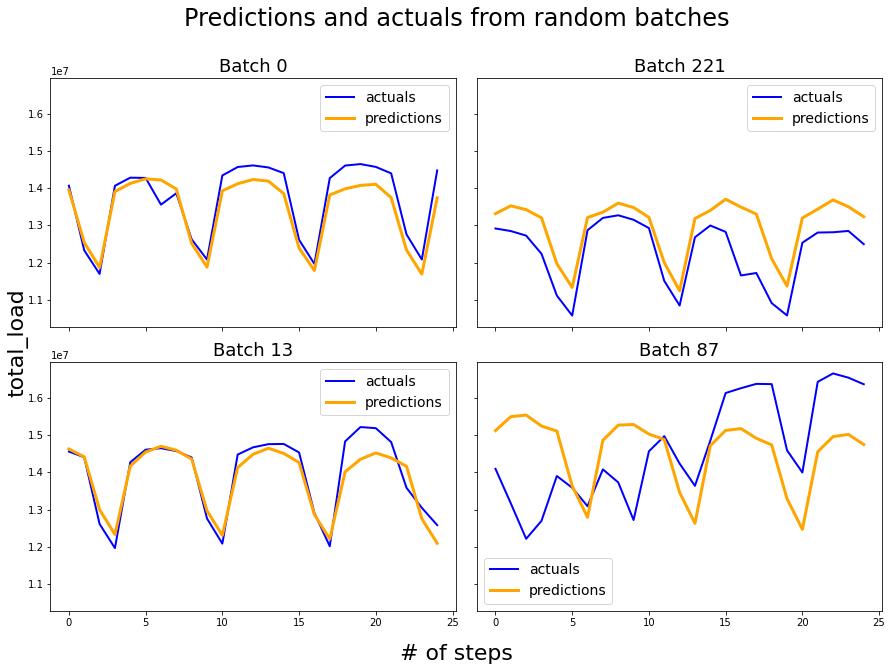
\includegraphics[width=0.9\textwidth]{RNNPlots/lstmpredictionsgood.png}
\caption{LSTM multi-step prediction of 25 days ahead, with look-back length of 50}
\label{fig:lstm_preds_1}
\end{figure}

Above is shown four different batches of the LSTM predictions and the corresponding actual values. What is interesting to note, is that it looks like the LSTM network has made some pretty good predictions, in most cases, the orange line is right on top of the blue. However, one could speculate that the model does not deviate much from the standard, as most of the predictions follow the same structure. This means that the model in this case is simply predicting around the mean values of the part of the data on which the predictions are based on. In the cases where there are anomalies or deviations from the mean in the actual data, the LSTM prediction fails to follow. This is very much the case in batch 87 for example.\\
This sentiment is also mirrored in the loss, where it can be seen from the plot below that the validation loss does not converge at all and even shows signs of overfitting. It should also be noted that the training ran for a relatively low number of epochs, even despite the fact that patience was set to 40, so after around 20 epochs, validation loss did not improve further for 40 epochs. Giving an indication that this model would not be able to learn very well.

\begin{figure}[H]
\centering
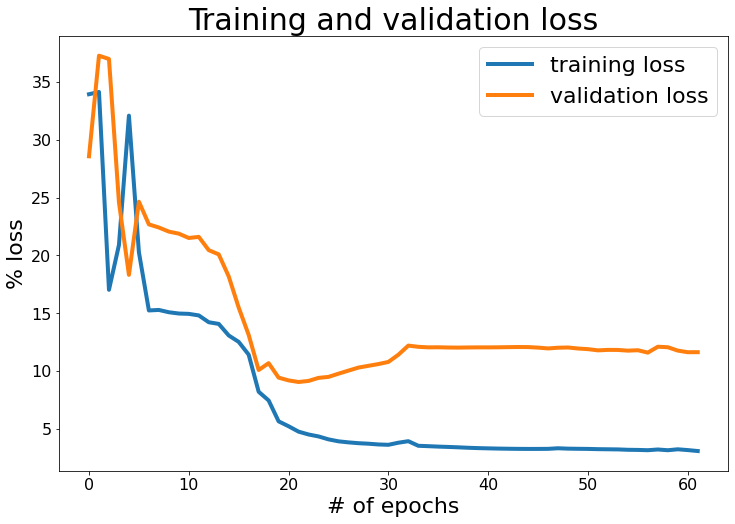
\includegraphics[width=0.6\textwidth]{RNNPlots/lstmloss25day.png}
\caption{}
\label{fig:lstm_loss_1}
\end{figure}

The missings of the LSTM model can furthermore be backed up by increasing the number of steps on which the model makes predictions to 50 days, where the point is emphasized, especially with batch 94 and 170 seen below.

\begin{figure}[H]
\centering
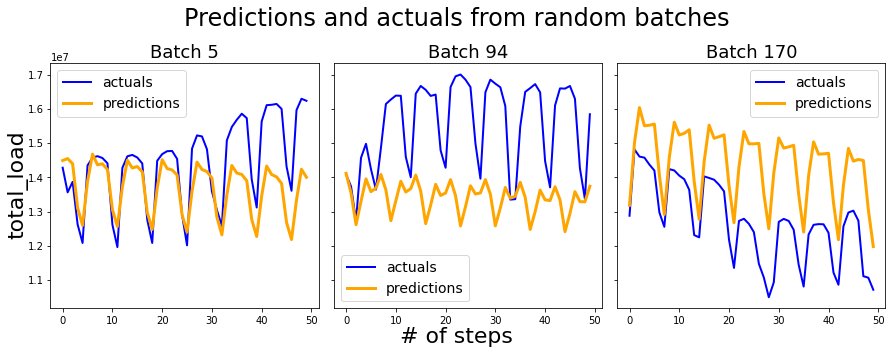
\includegraphics[width=0.9\textwidth]{RNNPlots/lstmpredictionsbad2.png}
\caption{LSTM multi-step prediction of 50 days ahead, with look-back length of 50}
\label{fig:lstm_preds_2}
\end{figure}

Lastly, to have another more quantitative and more direct point of comparison, the average distance between the predicted values and actuals values across batches are presented. Here the above sentiments are visualized where it can be seen that the predictions on average get worse and worse the longer the prediction sequence gets.

\begin{figure}[H]
    \centering
    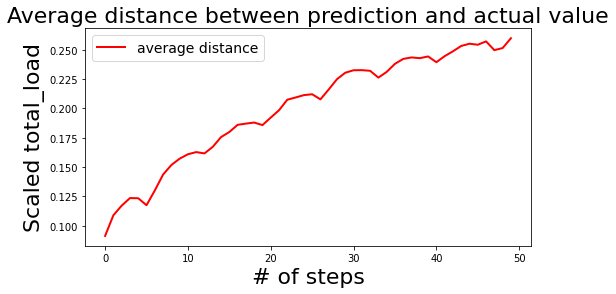
\includegraphics[width=0.7\textwidth]{RNNPlots/avgerrorlstm.png}
    \caption{Average distance between predicted and actual values for the LSTM model}
    \label{fig:avgerrorlstm}
\end{figure}

\end{document}